% Auto-generated TikZ AIG diagram
\documentclass[tikz,border=2mm]{standalone}
\usepackage{tikz}
\usetikzlibrary{shapes,arrows.meta,positioning}
\begin{document}
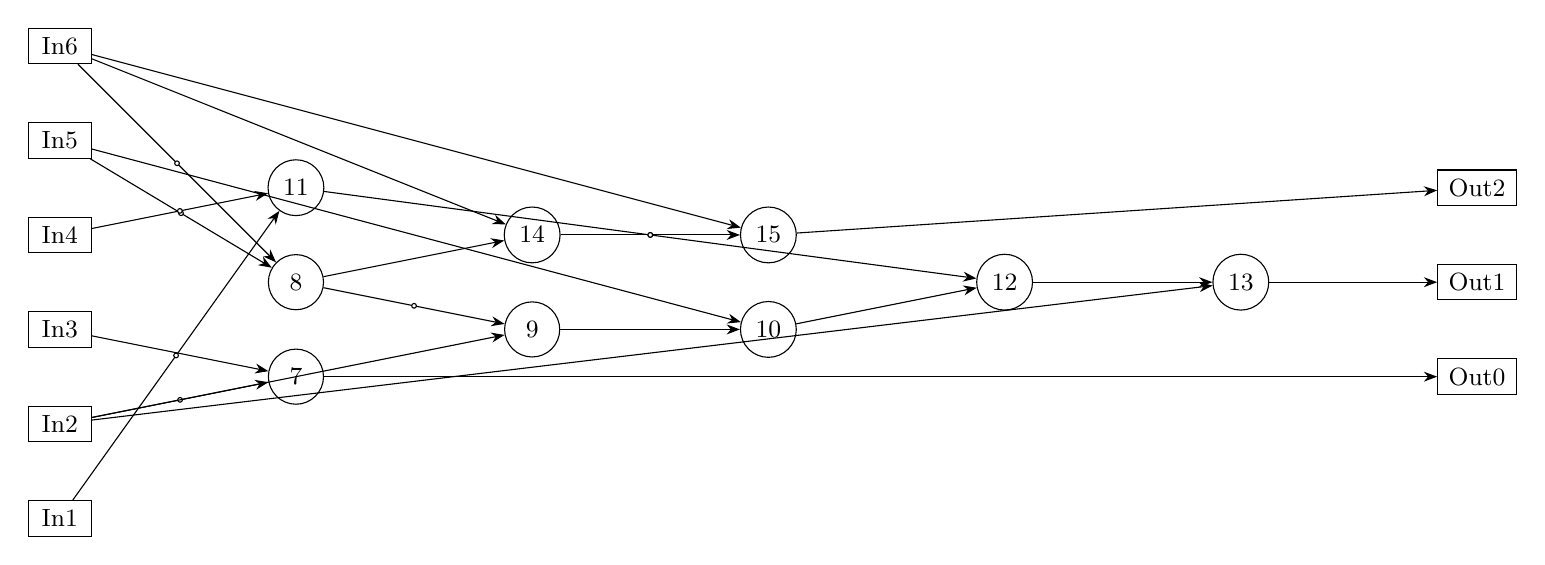
\begin{tikzpicture}[every node/.style={font=\small}, >=Stealth]

\node[draw, rectangle, minimum width=8mm, minimum height=4mm] (n1) at (0.000,-3.000) {In1};
\node[draw, rectangle, minimum width=8mm, minimum height=4mm] (n2) at (0.000,-1.800) {In2};
\node[draw, rectangle, minimum width=8mm, minimum height=4mm] (n3) at (0.000,-0.600) {In3};
\node[draw, rectangle, minimum width=8mm, minimum height=4mm] (n4) at (0.000,0.600) {In4};
\node[draw, rectangle, minimum width=8mm, minimum height=4mm] (n5) at (0.000,1.800) {In5};
\node[draw, rectangle, minimum width=8mm, minimum height=4mm] (n6) at (0.000,3.000) {In6};
\node[draw, circle, minimum size=7mm] (n7) at (3.000,-1.200) {7};
\node[draw, circle, minimum size=7mm] (n8) at (3.000,0.000) {8};
\node[draw, circle, minimum size=7mm] (n9) at (6.000,-0.600) {9};
\node[draw, circle, minimum size=7mm] (n10) at (9.000,-0.600) {10};
\node[draw, circle, minimum size=7mm] (n11) at (3.000,1.200) {11};
\node[draw, circle, minimum size=7mm] (n12) at (12.000,0.000) {12};
\node[draw, circle, minimum size=7mm] (n13) at (15.000,0.000) {13};
\node[draw, circle, minimum size=7mm] (n14) at (6.000,0.600) {14};
\node[draw, circle, minimum size=7mm] (n15) at (9.000,0.600) {15};
\draw[->] (n3) -- (n7);
\draw[->] (n2) -- node[midway,draw,circle,fill=white,inner sep=0.6pt] {} (n7);
\draw[->] (n6) -- node[midway,draw,circle,fill=white,inner sep=0.6pt] {} (n8);
\draw[->] (n5) -- node[midway,draw,circle,fill=white,inner sep=0.6pt] {} (n8);
\draw[->] (n8) -- node[midway,draw,circle,fill=white,inner sep=0.6pt] {} (n9);
\draw[->] (n2) -- (n9);
\draw[->] (n9) -- (n10);
\draw[->] (n5) -- (n10);
\draw[->] (n4) -- node[midway,draw,circle,fill=white,inner sep=0.6pt] {} (n11);
\draw[->] (n1) -- node[midway,draw,circle,fill=white,inner sep=0.6pt] {} (n11);
\draw[->] (n11) -- node[midway,draw,circle,fill=white,inner sep=0.6pt] {} (n12);
\draw[->] (n10) -- (n12);
\draw[->] (n12) -- (n13);
\draw[->] (n2) -- (n13);
\draw[->] (n8) -- (n14);
\draw[->] (n6) -- (n14);
\draw[->] (n14) -- node[midway,draw,circle,fill=white,inner sep=0.6pt] {} (n15);
\draw[->] (n6) -- (n15);
\node[draw, rectangle, minimum width=10mm] (out0) at (18.000,-1.200) {Out0};
\draw[->] (n7) -- (out0);
\node[draw, rectangle, minimum width=10mm] (out1) at (18.000,0.000) {Out1};
\draw[->] (n13) -- (out1);
\node[draw, rectangle, minimum width=10mm] (out2) at (18.000,1.200) {Out2};
\draw[->] (n15) -- (out2);

\end{tikzpicture}
\end{document}
